% Project-authored deployment workflow using named nodes and arrow colors.
% Syntax reference: https://tikz.dev/tikz-shapes and https://tikz.dev/tikz-arrows
\documentclass{article}
\usepackage{tikz}
\usetikzlibrary{arrows.meta,shapes.geometric}

\title{Release Gate and Rollback Workflow}
\author{Platform Reliability Team}
\date{September 2026}

\begin{document}
\maketitle

\section{From candidate to production}
A release candidate passes automated tests and a canary deployment before
general rollout. A failed canary triggers rollback and a defect review; a
healthy canary proceeds to production and post-release monitoring. The
diagram places each stage at an explicit coordinate so the two outcomes of
each decision remain visible.

\begin{figure}
\centering
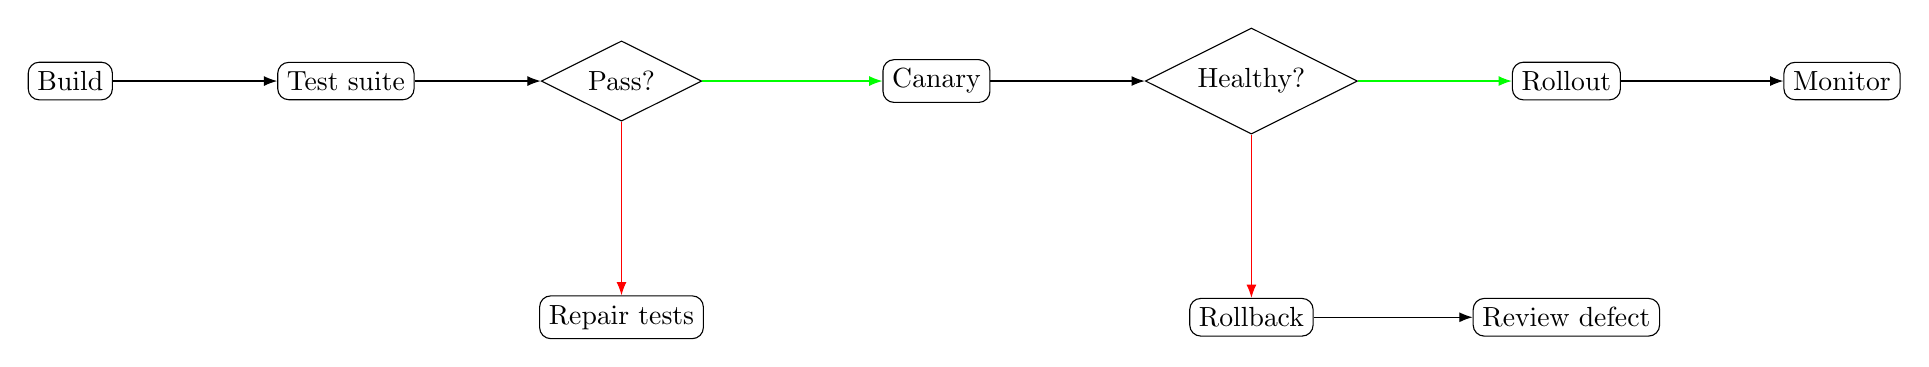
\begin{tikzpicture}
  \node[draw,rounded corners] (build) at (0,0) {Build};
  \node[draw,rounded corners] (tests) at (3.5,0) {Test suite};
  \node[draw,diamond,aspect=2] (gate) at (7,0) {Pass?};
  \node[draw,rounded corners] (canary) at (11,0) {Canary};
  \node[draw,diamond,aspect=2] (health) at (15,0) {Healthy?};
  \node[draw,rounded corners] (rollout) at (19,0) {Rollout};
  \node[draw,rounded corners] (monitor) at (22.5,0) {Monitor};
  \node[draw,rounded corners] (repair) at (7,-3) {Repair tests};
  \node[draw,rounded corners] (rollback) at (15,-3) {Rollback};
  \node[draw,rounded corners] (review) at (19,-3) {Review defect};
  \draw[-{Latex}] (build) -- (tests);
  \draw[-{Latex}] (tests) -- (gate);
  \draw[green,-{Latex}] (gate) -- (canary);
  \draw[-{Latex}] (canary) -- (health);
  \draw[green,-{Latex}] (health) -- (rollout);
  \draw[-{Latex}] (rollout) -- (monitor);
  \draw[red,-{Latex}] (gate) -- (repair);
  \draw[red,-{Latex}] (health) -- (rollback);
  \draw[-{Latex}] (rollback) -- (review);
\end{tikzpicture}
\caption{Release stages with success and failure paths.}
\label{fig:release-gates}
\end{figure}

Green arrows represent promotion. Red arrows lead to remediation, keeping the
failure path distinct from the main delivery line.
\end{document}
